\chapter{数据库设计}
\section{数据库环境说明}
本系统的数据系统采用MySQL数据库系统。

\section{数据库的命名规则}
只有标识符“ID”可以缩写,其他有意义的名词不允许缩写

表名统一用单数。命名最大字节数为100,关联表用该表"ID"作为外键

统一所有表无前缀

\section{逻辑设计}
数据库设计应满足BCNF范式

实体的逻辑关系图如下
\begin{figure}
    \centering
    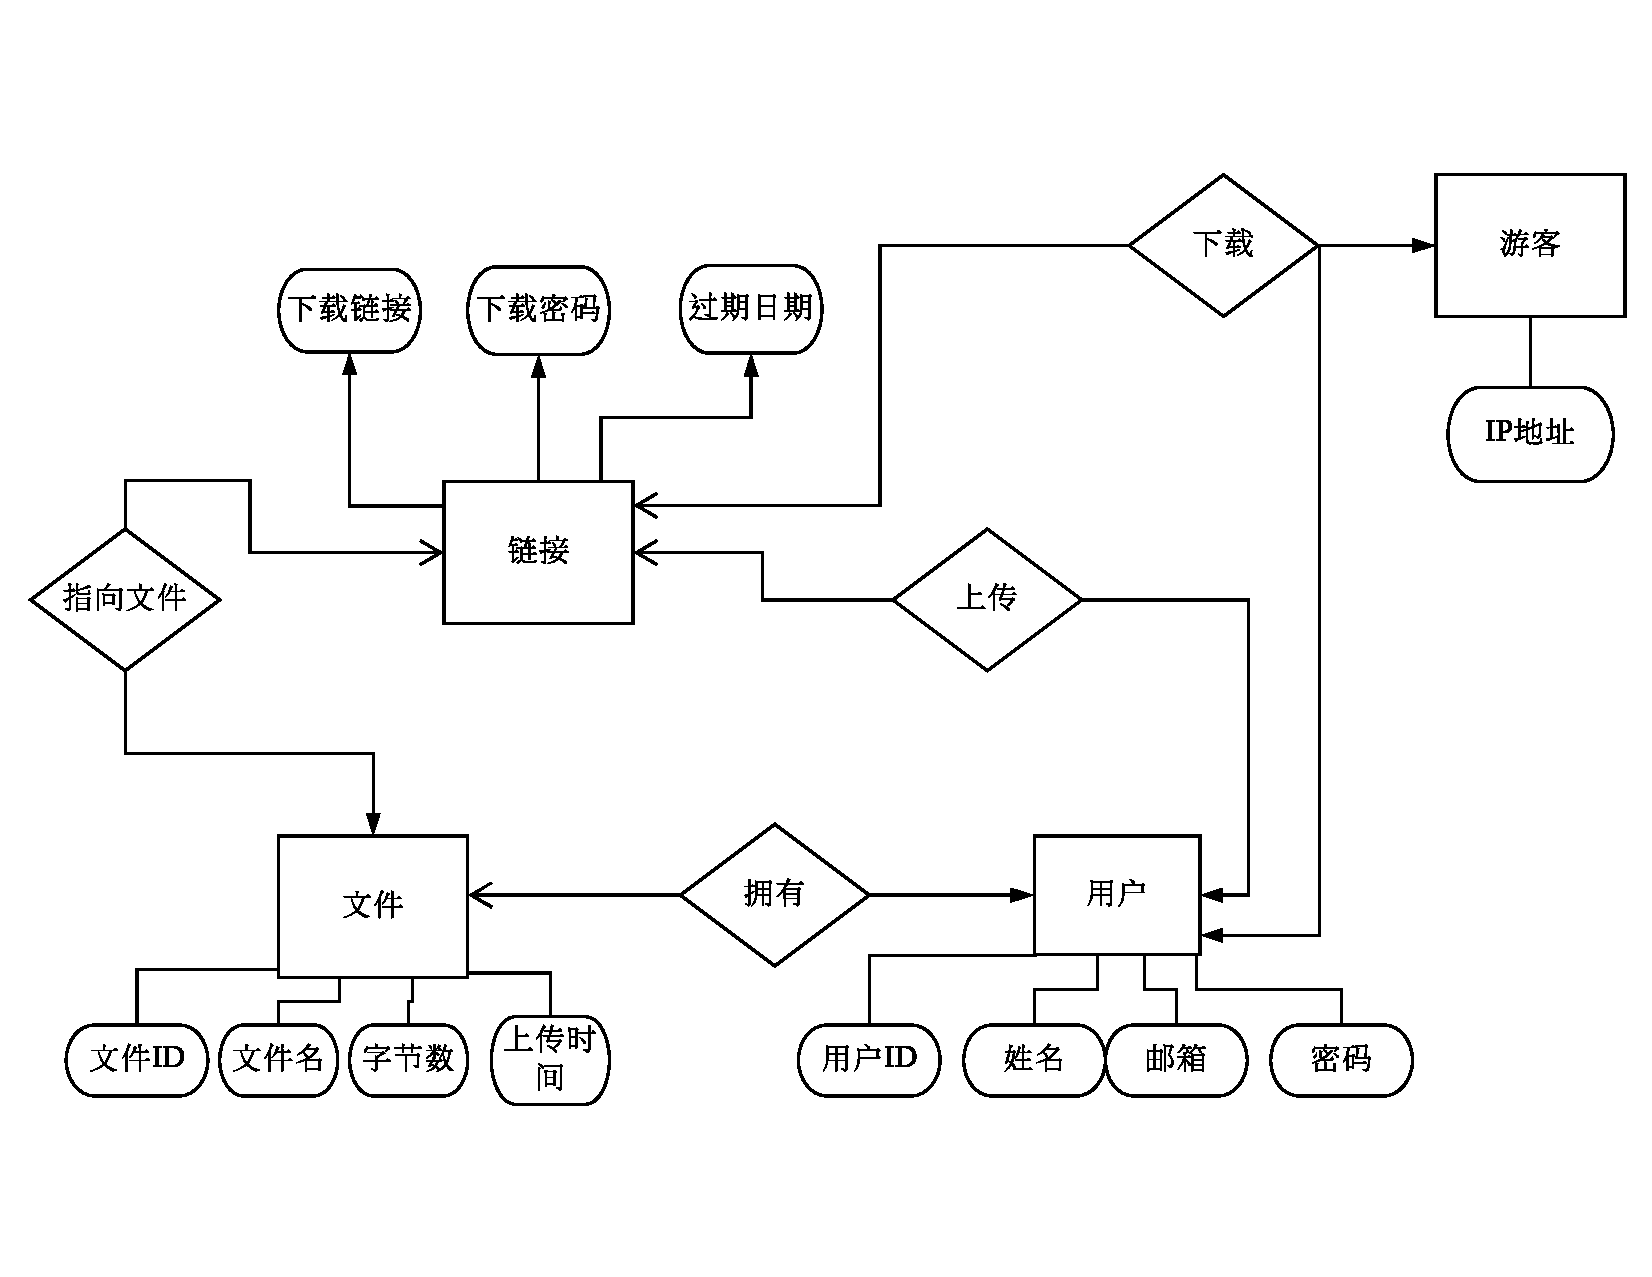
\includegraphics[width=16cm]{ER.pdf}
    \caption{ER关系图}\label{fig:noted-figure}
\end{figure}

\section{物理设计}
\subsection{数据库产品}
数据库采用MySql数据库。
由于文件本身是存储在ceph中的,数据库只存储控制信息,因此不需要分布式数据库。
数据库所在的服务器应使用 1TB 以上的 SSD 硬盘并使用 32G 以上内存

\subsection{实体属性、类型、精度}
\subsubsection{文件数据表设计}
\begin{table}[htbp]
\centering
\caption{文件数据表Files设计} \label{tab:file-database}
\begin{tabular}{|c|c|c|c|c|}
    \hline
    字段名 & 类型 & 大小 & 说明 & 备注 \\
    \hline
    文件ID & char & 64 & 文件的唯一标识符 & 主键\\
    \hline
    文件路径 & char & 512 & 文件在用户目录下路径 & \\
    \hline
    文件模式 & char & 20 & 文件的信息(是否可写,可执行等)& \\
    \hline
    用户ID & char & 64 & 该文件拥有者的ID & 外键,来自User表 \\
    \hline
    字节数 & int & 1 & 文件大小 & \\
    \hline
    更新时间 & char & 64 & 上次上传文件更新的时间 & \\
    \hline
\end{tabular}
\note{文件数据表Files设计}
\end{table}

\subsubsection{用户数据表设计}
\begin{table}[htbp]
\centering
\caption{用户数据表Users设计} \label{tab:user-database}
\begin{tabular}{|c|c|c|c|c|}
    \hline
    字段名 & 类型 & 大小 & 说明 & 备注 \\
    \hline
    用户ID & char & 64 & 用户的唯一标识符 & 主键\\
    \hline
    用户名 & char & 64 & 对应用户 & \\
    \hline
    密码 & char & 64 & 用户登录的密码 & \\
    \hline
    邮箱地址 & char & 64 & 用户的邮箱 & \\
    \hline
    拥有的文件 & char & 512 & 该用户在云盘上所有的文件ID & \\
    \hline
\end{tabular}
\note{用户数据表Users设计}
\end{table}

\subsubsection{链接数据表设计}
\begin{table}[htbp]
\centering
\caption{链接数据表Users设计} \label{tab:link-database}
\begin{tabular}{|c|c|c|c|c|}
    \hline
    字段名 & 类型 & 大小 & 说明 & 备注 \\
    \hline
    用户ID & char & 64 & 对应用户 & 主键;外键,来自Users表\\
    \hline
    文件ID & char & 64 & 对应文件 & 主键;外键,来自Files表\\
    \hline
    链接网址 & char & 64 & 本链接的URL & \\
    \hline
    下载密码 & char & 64 & 输入密码下载资源 & \\
    \hline
    过期日期 & char & 128 & 链接失效的日期时间 & \\
    \hline
\end{tabular}
\note{链接数据表Links设计}
\end{table}

\section{安全性设计}
数据库每小时进行备份,并导出数据到备份服务器上。

数据库所在的磁盘使用带冗余的磁盘阵列。

数据库使用普通权限用户进行权限控制,设定数据表的读写权限。

\section{数据库管理与维护说明}
数据库的具体备份、压缩功能的实现主要交由 MySQL 的功能来完成。

备份的主要策略为:每次操作由主数据库完成之后,备份数据库向主数据库 fetch 更新。备份的恢复方式为将备份数据库的内容 copy 到主数据库。

对于文件系统的备份,由 ceph 这一高可用的文件系统来完成,其内部已有 replication 以及灾害恢复的功能,无需在外部另作备份。